\begin{flushright} {\tiny {\color{gray} basis\_p2p\_3D.tex}} \end{flushright}
%~~~~~~~~~~~~~~~~~~~~~~~~~~~~~~~~~~~~~~~~~~~~~~~~~~~~~~~~~~~~~~~~~~~~~~~~~~~~~~~~~~~~~~~~~~~~~~~~~~

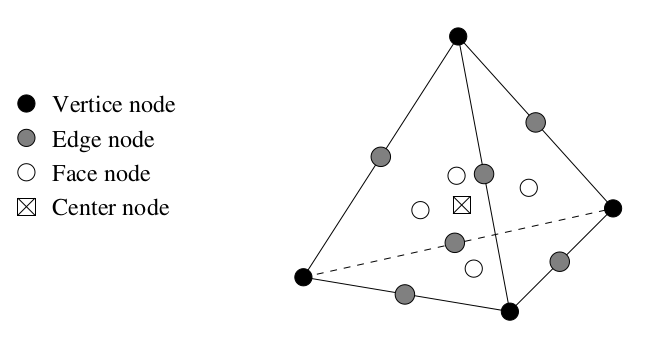
\includegraphics[width=9cm]{images/crouzeix-raviart/p2pp1_3D1}
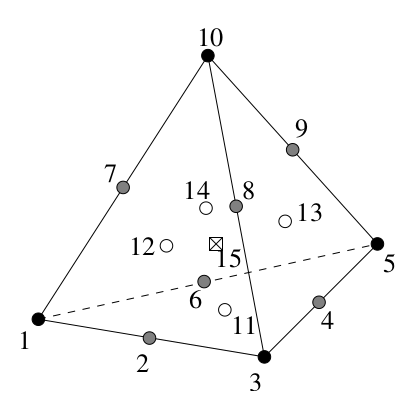
\includegraphics[width=5cm]{images/crouzeix-raviart/p2pp1_3D2}

The velocity basis functions are:
\begin{eqnarray}
\phi_i &=& \lambda_i(2\lambda_i-1) + 3 (\lambda_i\lambda_j \lambda_k + \lambda_i\lambda_j\lambda_l + \lambda_i\lambda_k\lambda_l) -4 \lambda_i\lambda_j\lambda_k\lambda_l \\
\phi_{ij} &=& 4\lambda_i\lambda_j - 12( \lambda_i\lambda_j\lambda_k+\lambda_i\lambda_j\lambda_l  ) +32 \lambda_i\lambda_j\lambda_k \lambda_l \\
\phi_{ijk} &=& 27  \lambda_i\lambda_j\lambda_k - 108 \lambda_i\lambda_j\lambda_k \lambda_l \\
\phi_c &=& 256 \lambda_i\lambda_j\lambda_k\lambda_l
\end{eqnarray}

\todo[inline]{REFS ??? better definition of functions !}
